%class
	\documentclass{beamer}

%template
	\usetheme{HannoverSalman}
	\setbeamertemplate{navigation symbols}{}
	%\setbeamertemplate{footline}{\centering{\insertframenumber/\insertpresentationendpage}}
	%\setbeamertemplate{footline}{\hspace*{.5cm}\scriptsize{\hfill\insertframenumber\hspace*{.5cm}}} 


%packages
	\usepackage{amsmath, amssymb, graphicx,cancel}
	\usepackage[absolute,overlay]{textpos}
	\usepackage{subfigure}
	\usepackage{caption}\captionsetup{labelformat=empty,labelsep=none}
	\usepackage{geometry}
	\geometry{verbose}
	\usepackage{color}
	\usepackage{xmpmulti}
	\usepackage[3D]{movie15}
	\usepackage{hyperref}
%	\usepackage{bookmark}
	\usepackage[open,openlevel=4,atend]{bookmark}
	%\bookmarksetup{color=blue}
	\usepackage{multirow}
	\usepackage[style=numeric,defernumbers, authoryear]{biblatex}
	%\usepackage[square,sort]{natbib}
	%\usepackage{fancyhdr}%\pagestyle{fancy} 

	
	\hypersetup{bookmarksdepth = 4}


%citations files
	\bibliography{MyCitations}

%logoCSIPCPL
    \setlength{\TPHorizModule}{1mm}
    \setlength{\TPVertModule}{1mm}
    \newcommand{\logoCSIPCPL}
    {
    	\begin{textblock}{1}(100,2) %(100,85)  for bottom
    		
\includegraphics[width=1.5cm]{figs/logo_CSIP}
    	\end{textblock}
    	
	\begin{textblock}{1}(117,1) %(117,85)  for bottom
    		
\includegraphics[width=1.0cm]{figs/logo_CPL}
    	\end{textblock} 
    }

%logo evolution
    \newcommand{\logoEvolution}
    {    	
	\begin{textblock}{1}(110,1) %(117,85)  for bottom
    		\includegraphics[width=0.65in]{figs/logo_evolution.pdf}
    	\end{textblock} 
    }

%logo Qualcomm
    \newcommand{\logoQualcomm}
    {
    	\begin{textblock}{1}(110,2) %(100,85)  for bottom
    		\includegraphics[width=1.5cm]{figs/logo_qualcomm.jpg}
    	\end{textblock}
    }
%logo Qualcomm (long)
    \newcommand{\logoQualcommllong}
    {
    	\begin{textblock}{1}(0,0) 
    		\includegraphics[width=1.25in]{figs/logo_qualcomm_long.jpg}
    	\end{textblock}
    }

%logo Tech Tower
    \newcommand{\logoTechTower}
    {
    	\begin{textblock}{1}(0,0) 
    		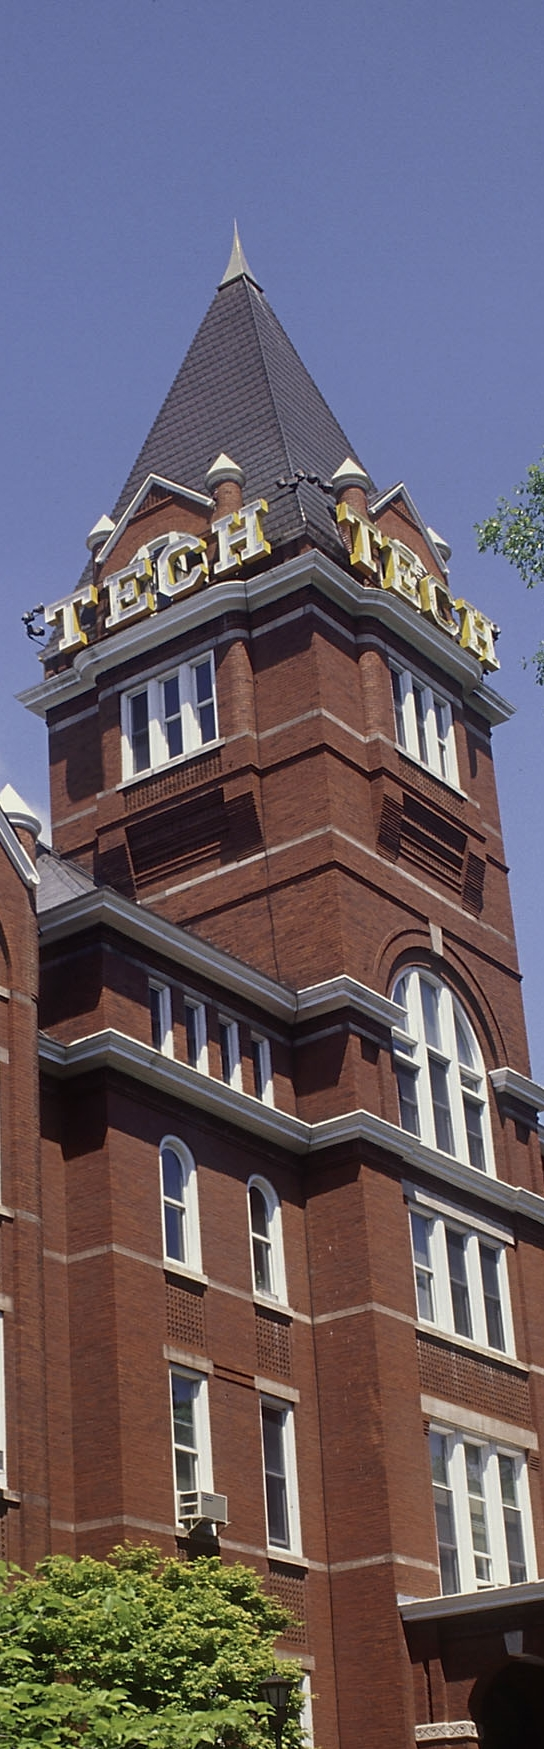
\includegraphics[width=1.25in]{figs/logo_TechTower.jpg}
    	\end{textblock}
    }

%logo tree
    \newcommand{\logoTree}
    {
    	\begin{textblock}{1}(0,0) 
    		\includegraphics[width=1.25in]{figs/logo_tree.jpg}
    	\end{textblock}
    }
%page numbers
    \newcommand{\mypagenum}
    {
    	\begin{textblock}{1}(1,94) 
		{\tiny \color[rgb]{0.2,0.2,1}\insertframenumber} %\insertframenumber,\insertpresentationendpage, \inserttotalframenumber
    	\end{textblock}
    }
%my footnote citation
	\newcommand{\myFootnoteCitation}[2]
	{
		\footnote{\tiny \citeauthor{#1}, \emph{#2}, \citeyear{#1}.}  %\citeauthor{#1}, \citetitle{#1}, #2 \citeyear{#1}.
	}
%my refer to citation
	\newcommand{\mycite}[1]
	{
		\emph{\citeauthor{#1} (\citeyear{#1})}
	}
%my footnote website citation
	\newcommand{\myFootnoteWebsiteCitation}[1]
	{
		\footnote{\tiny \citeauthor{#1}}
	}

\let\thefootnote\relax\footnotetext{Footnotetext without footnote mark}


%section underline
%\newcommand{\tmpsection}[1]{}
%\let\tmpsection=\section
%\renewcommand{\section}[1]{\tmpsection{\underline{#1}}}



%commands
	\newcommand{\likelihood}{p(Z_k| x_k) }						%likelihood
	\newcommand{\prior}{p(x_k)  } 								%prior
	\newcommand{\posterior} {p(x_k| Z_k)}						%posterior
	\newcommand{\prediction} {p(x_k| Z_{k-1})}					%prediction
	\newcommand{\update} {p(x_k|Z_k)}							%update
	\newcommand{\observations} {p(Z_k)}						%observations
	\newcommand{\prevobservations} {p(Z_{k-1})}				%previous observations
	\newcommand{\dxpk} {dx_{k-1}}							%dx_{k-1}
	\newcommand{\ChapKolm}{\int{p(x_k| x_{k-1})p(x_{k-1}|Z_{k-1})} \dxpk} %Chapman Kolmogorov

	%algorithm specific: JPDAF
	\newcommand{\likelihoodJPDAF}{p(Z_k| \chi, m, Z_{k-1}) }		%1. likelihood
	\newcommand{\priorJPDAF}{p(\chi|m, Z^{k-1}} 				%2. prior	
	\newcommand{\observationsJPDAF} {p(Z_k}					%3. observations
	\newcommand{\posteriorJPDAF} {p(\chi| Z_k)}					%4. posterior

%environments
	\newenvironment{changemargin}[2]
	{
	  	\begin{list}{}
		{
			\setlength{\topsep}{0pt}%
			\setlength{\leftmargin}{#1}%
			\setlength{\rightmargin}{#2}%
			\setlength{\listparindent}{\parindent}%
			\setlength{\itemindent}{\parindent}%
			\setlength{\parsep}{\parskip}%
		}
	  	\item[]
		}
		{\end{list}
	}
%figures

%colors
\definecolor{darkgreen}{rgb}{0,0.5,0}

%personal details
	\author{Salman Aslam}
	\institute{Advisor, Dr Christopher Barnes (ECE)\\Co-advisor, Dr Aaron Bobick (CoC)\\Georgia Institute of Technology}
	\date{}

\begin{document}
%####################################################################################################
\title{Compensation Methods Using \\Signal Processing \\And \\Adaptive Quantization \\For Better Mean Shift Tracking On Compressed Video}
%####################################################################################################
\begin{frame}[plain]\logoTechTower
	\titlepage
\end{frame}


\begin{frame}\frametitle{Outline}\logoTechTower\logoCSIPCPL\mypagenum
	\tableofcontents
\end{frame}




%####################################################################################################
\section{Introduction}
%####################################################################################################
\begin{frame}
\frametitle{Introduction}
\framesubtitle{goal}
\logoCSIPCPL\mypagenum
	We want to run some computer vision algorithm (e.g. tracking) on compressed video.
	\begin{itemize}
		\item We would like the results of the algorithm (e.g. track positions) to be as close as possible to results generated if the algorithm were run on uncompressed video.
	\end{itemize}
	\begin{figure}		
		\includegraphics[width=0.9\textwidth]{figs/ICIP2009_ProblemStatement.pdf}
	\end{figure}
\end{frame}




%===================================
\subsection{Possible solutions}
%===================================
\begin{frame}
\frametitle{Introduction}
\framesubtitle{possible solutions}
\logoCSIPCPL\mypagenum
	\begin{enumerate}
		\item Codec based solution
			\begin{itemize}
				\item custom codec
				\item standard codec
					\begin{itemize}
						\item metadata support, e.g. MPEG-4
						\item intelligently vary quantization parameter $Q_p$, or quantization matrices
					\end{itemize}
			\end{itemize}
		\item Signal processing based solution
			\begin{itemize}
				\item Vary input signal intelligently to make it robust to degradations in the encoding/decoding process
			\end{itemize}
			\begin{figure}
				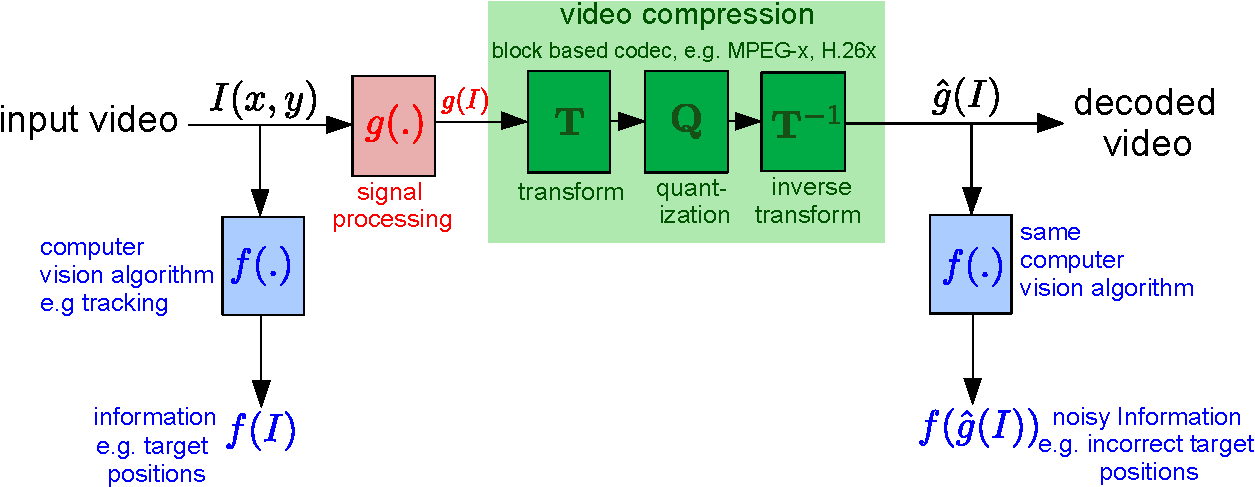
\includegraphics[width=0.9\textwidth]{figs/ICIP2009_SolutionThroughSigProc.pdf}
			\end{figure}
	\end{enumerate}
\end{frame}



%===================================
\subsection{Our approach}
%===================================
\begin{frame}
\frametitle{Introduction}
\framesubtitle{our approach} 
\logoCSIPCPL\mypagenum
	{\color{red}Varying quantization parameter $Q_p$}
	\begin{figure}
		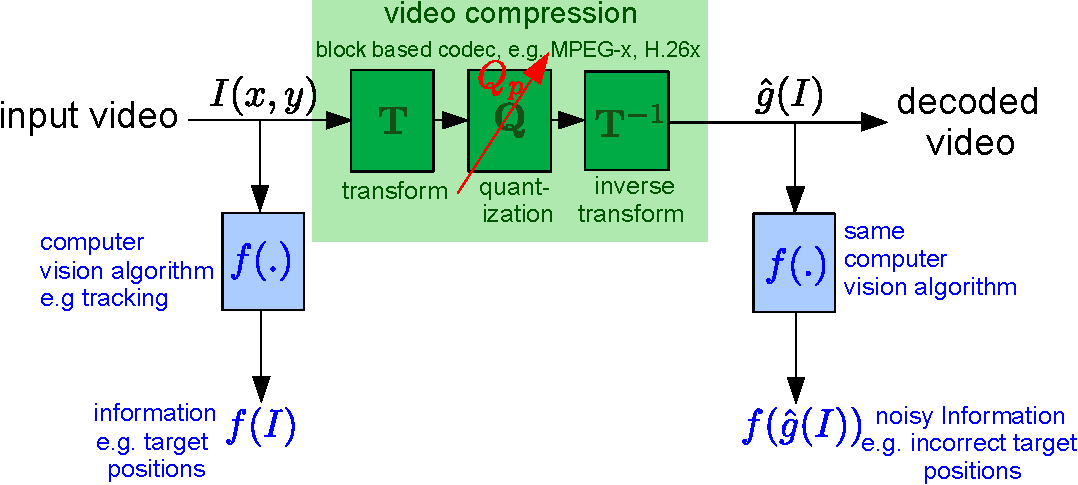
\includegraphics[width=1.0\textwidth]{figs/TRK_IPCV2009_BlockDiagram_2_VarPar_2.pdf}
	\end{figure}
\end{frame}



%===================================
\subsection{Theoretical background}
%===================================
\begin{frame}
\frametitle{Introduction}
\framesubtitle{mean shift filtering: notation}
\logoCSIPCPL\mypagenum
	\begin{itemize}
		\item {\color{red}$N$}: number of data points
		\item {\color{red}$D$}: number of dimensions
	 	\item {\color{red}$p(x)$}: distribution of {\color{red}$x$}
		\item {\color{red}$R$}: small region containing {\color{red}$K$} data points (a subset of all the data points in $x$)
		\item {\color{red}$V$}: volume of $R$
		\item {\color{red}$P$}: each point in $x$ has probability $P$ of falling in $R$, where
			\begin{equation*}
				P=\int_R p(x)dx
			\end{equation*}
		\item {\color{red}\text{bin}$(K|N,P)$}: binomial distribution for $K$
		\item {\color{red} $k(u)$}: unit square centered on origin, a Parzen window
			\begin{equation*}
				k(u) = 
				\left\{ 
				\begin{array}{rl}
					1\text{,} &  |u_i|<1/2 \ \ \ \ \ \ \ \ \ i=1,\ldots, D\\ 
					0\text{,} &  \mbox{otherwise}
				\end{array}
				\right.
			\end{equation*}
	\end{itemize}
\end{frame}




\begin{frame}
\frametitle{Introduction}
\framesubtitle{mean shift filtering: adaptive gradient ascent}
\logoCSIPCPL\mypagenum
	\begin{figure}				
		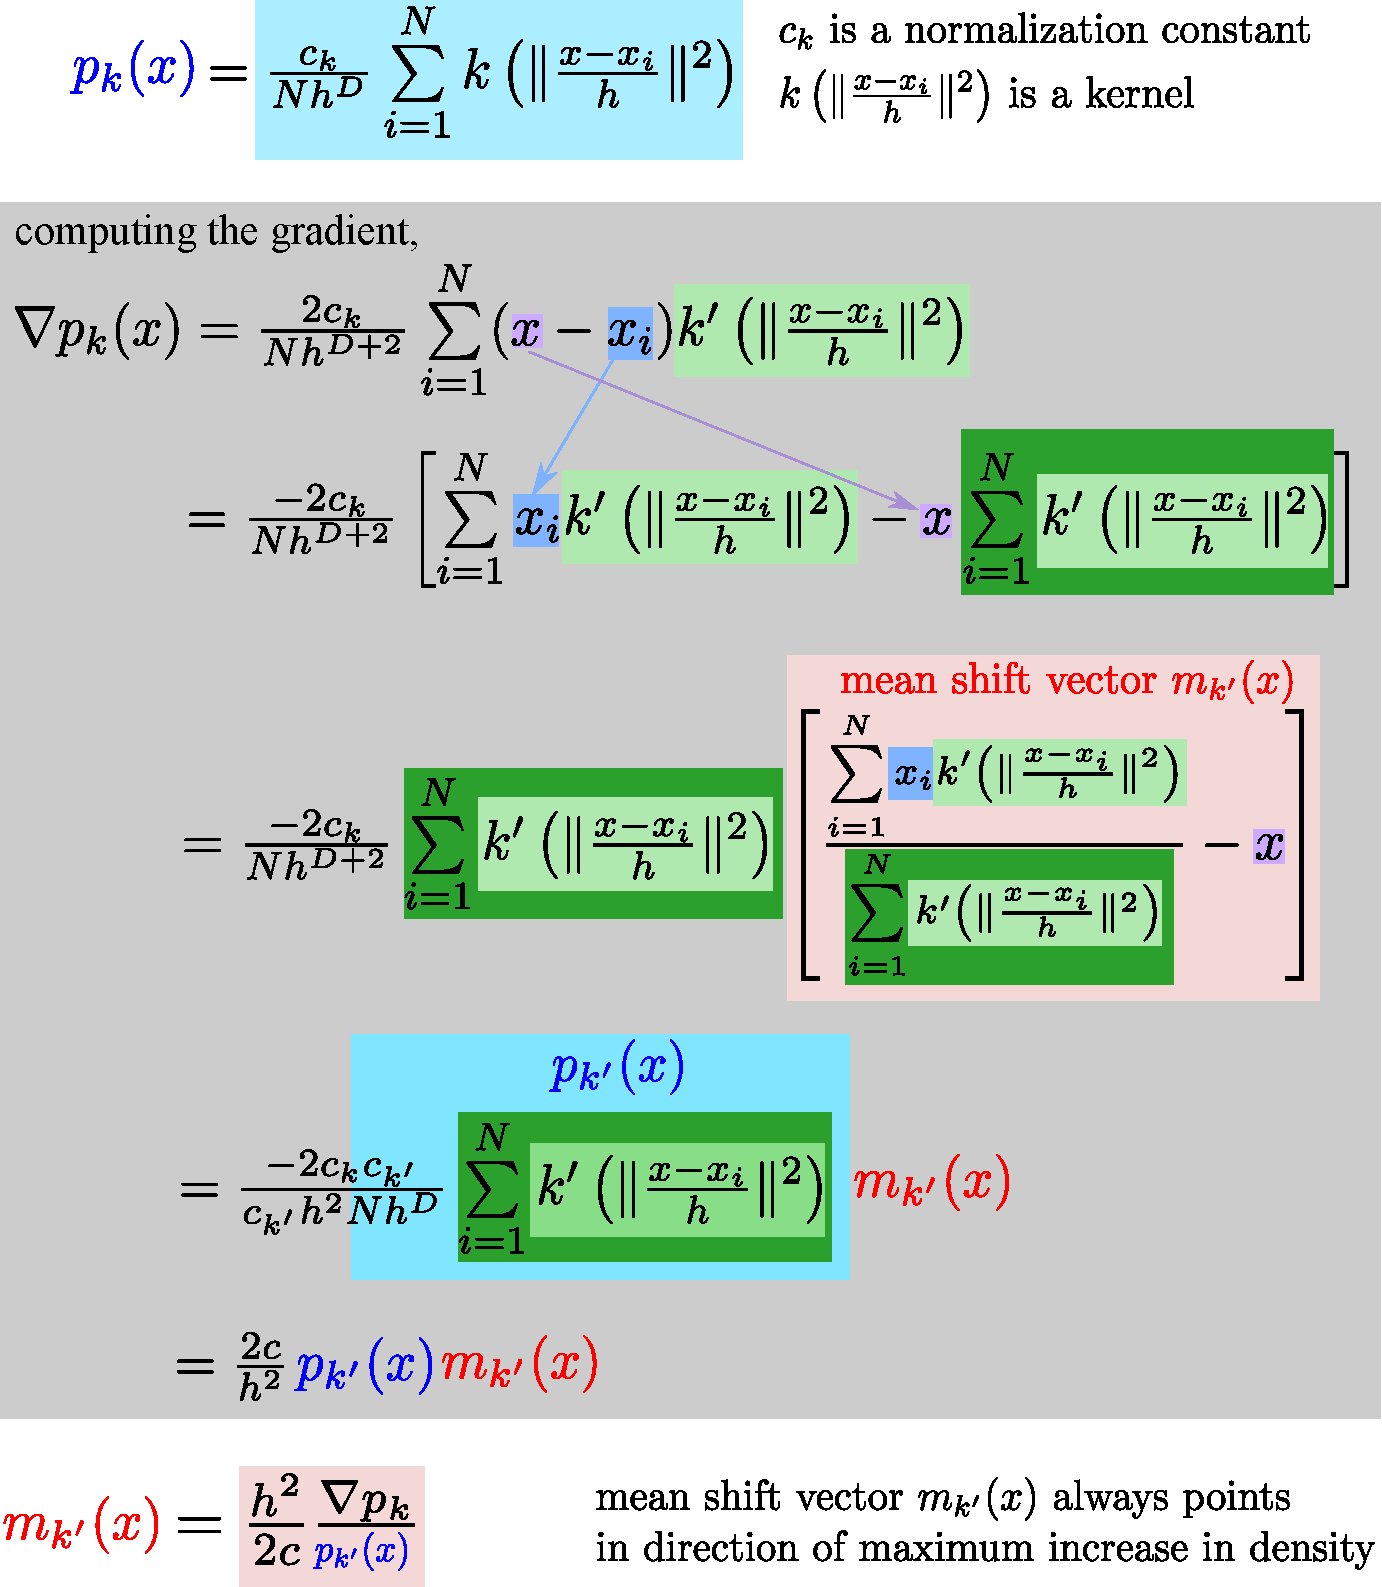
\includegraphics[height=.85\textheight]{figs/PRML_meanShift.pdf}
	\end{figure}
\end{frame}





\begin{frame}
\frametitle{Introduction}
\framesubtitle{mean shift filtering: simplification with uniform kernel}
\mypagenum
	New target center, $x_c$ and $y_c$ are computed as,
	\begin{align*}
		\label{eq:MeanShiftEquations}
		M_{00}&=\sum_x\sum_yI(x,y)		\\
		M_{10}&=\sum_x\sum_yxI(x,y)		\\
		M_{01}&=\sum_x\sum_yyI(x,y)		\\
		x_c&=\frac{M_{10}}{M_{00}}		\\
		y_c&=\frac{M_{01}}{M_{00}}
	\end{align*}
\end{frame}





%####################################################################################################
\section{Experiments}
%####################################################################################################

\begin{frame}
\frametitle{Experimental Setup}
\logoCSIPCPL\mypagenum 
	\begin{figure}
		\includegraphics[width=1.0\textwidth]{figs/TRK_IPCV2009_ExperimentalSetup.pdf}
	\end{figure}
\end{frame}



%####################################################################################################
\section{Results}
%####################################################################################################
\begin{frame}
\frametitle{Results}
\framesubtitle{PETS2001} 
\logoCSIPCPL\mypagenum
	\begin{itemize}
		\item person tracking
		\item sparse background
		\item target occluded by object (car) with similar color distribution
	\end{itemize}
	\begin{figure}
		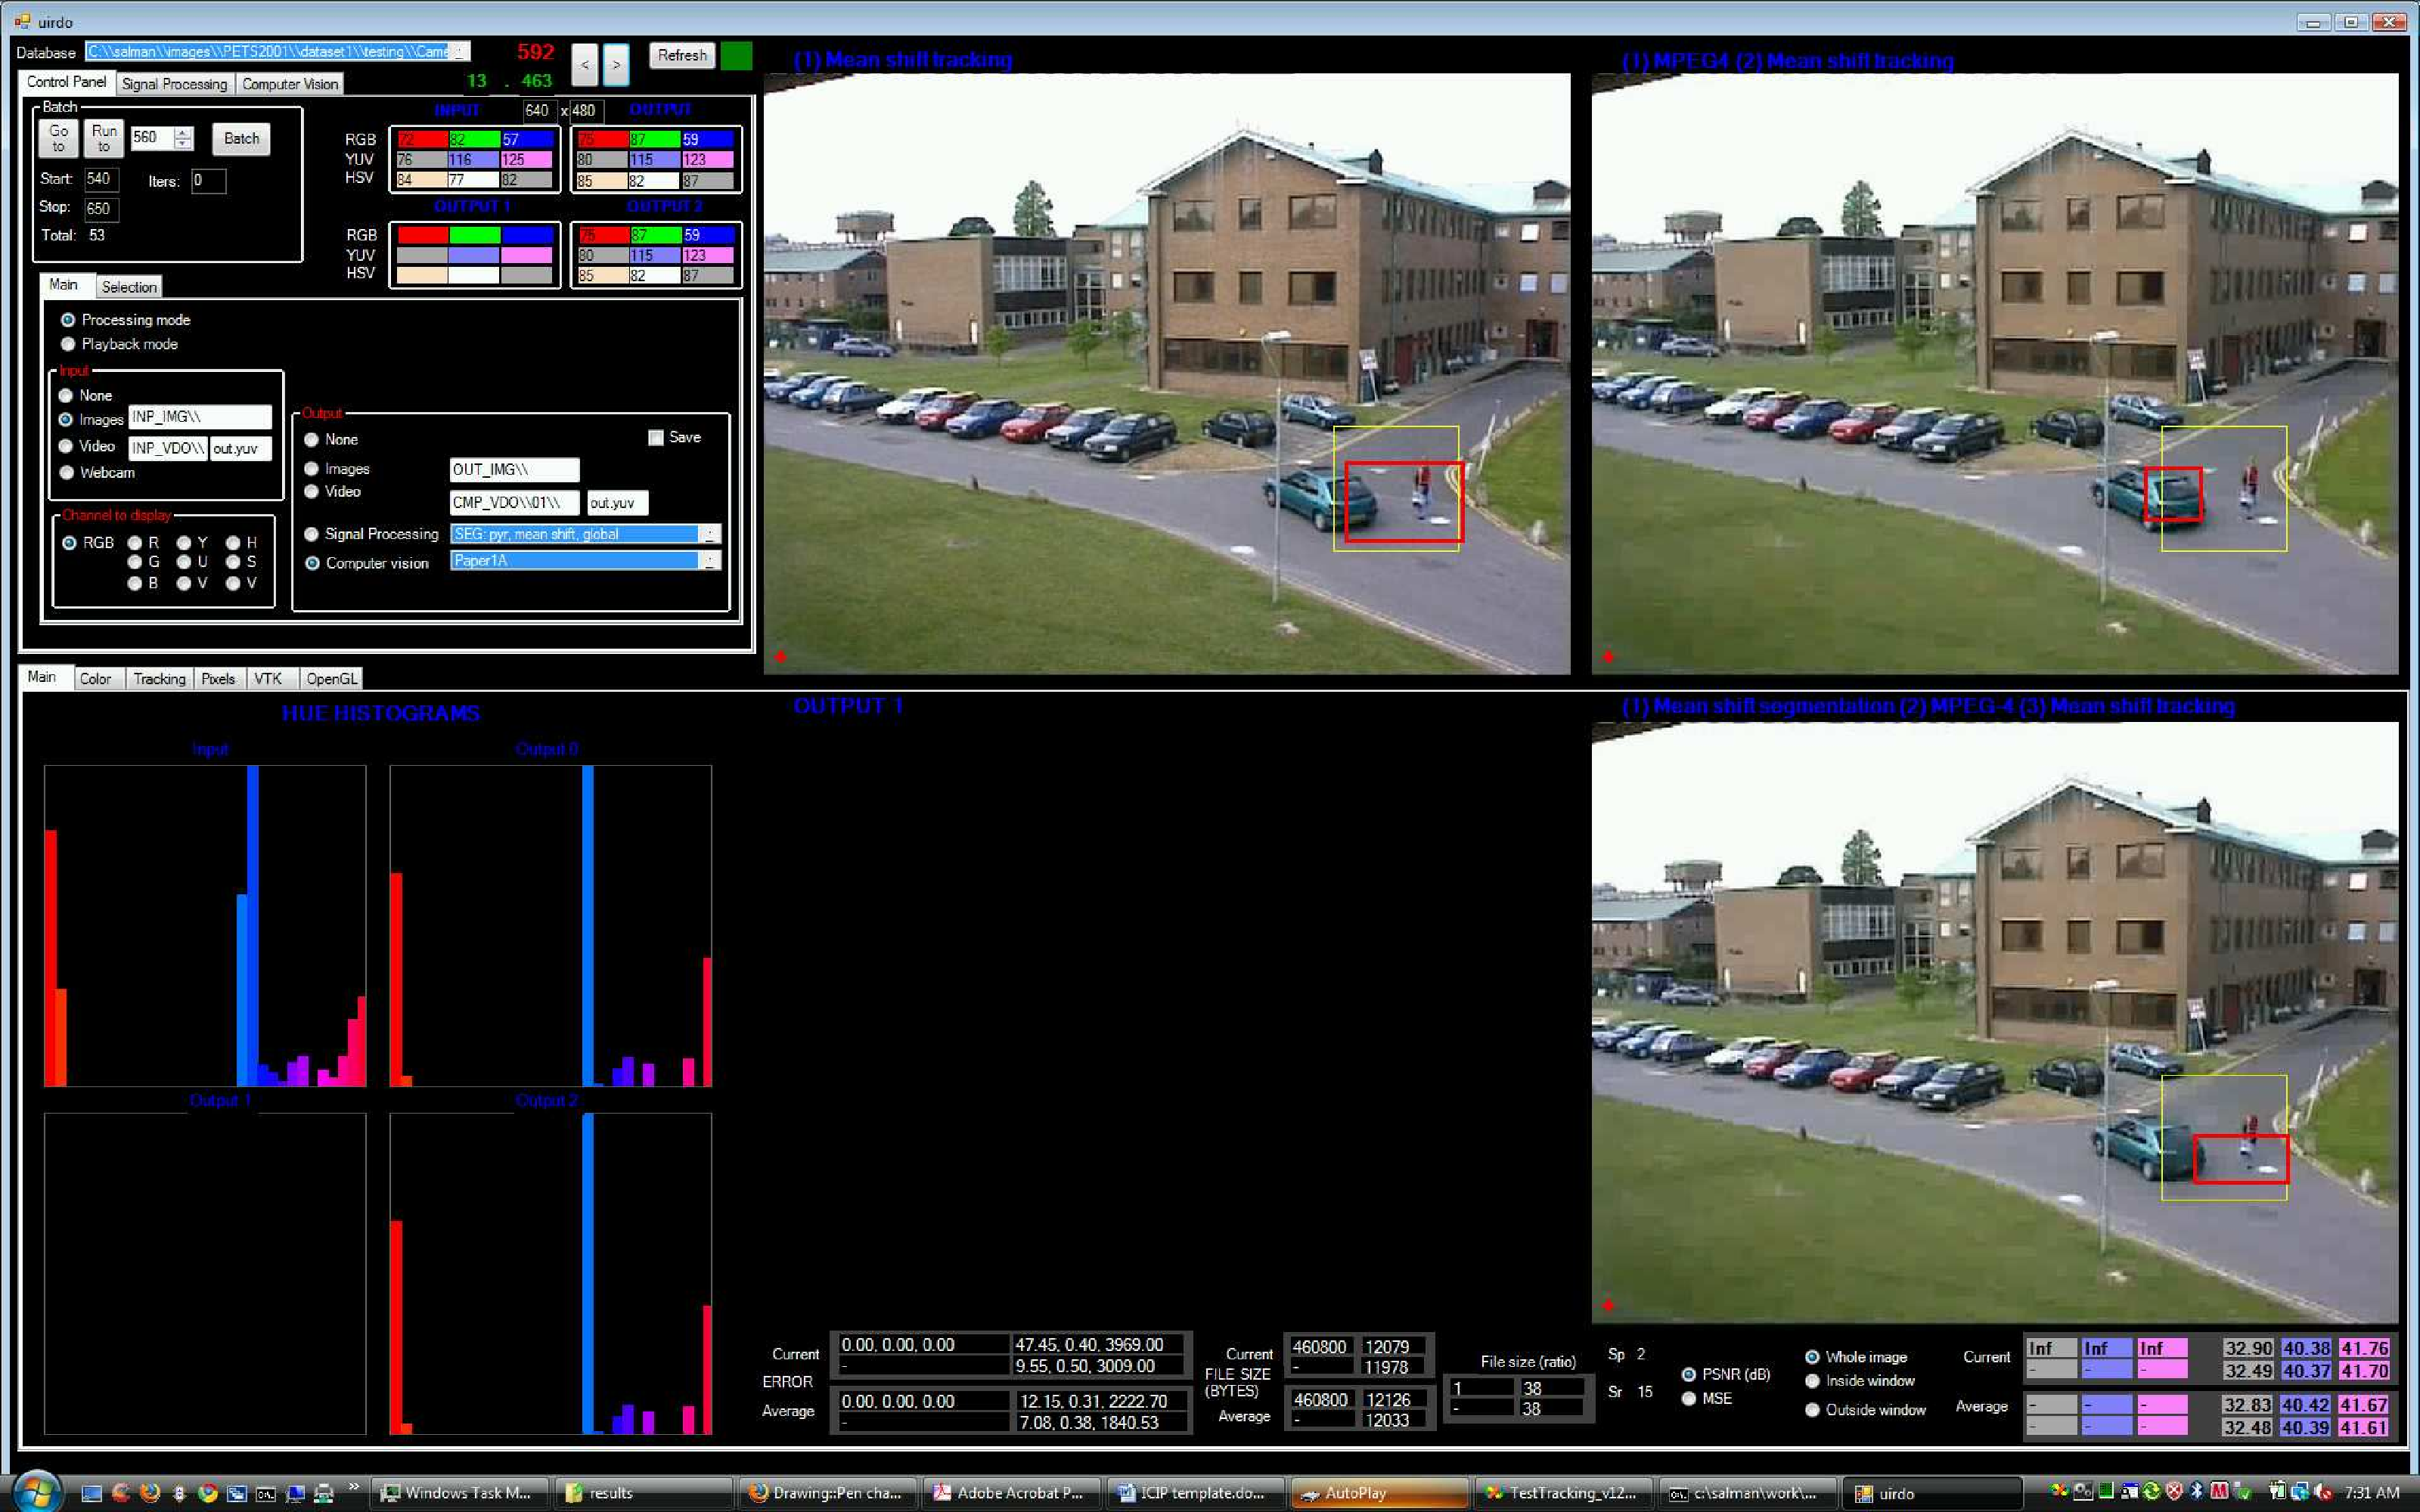
\includegraphics[width=1.0\textwidth]{figs/ICIP2009_PETS2001_FN_00592_snapshotVVG.pdf}
	\end{figure}
\end{frame}


\begin{frame}
\frametitle{Results}
\framesubtitle{PETS2001 (cont.)} 
\logoCSIPCPL\mypagenum
	\begin{figure}
		\centering
		\subfigure[Ground truth]
			{
				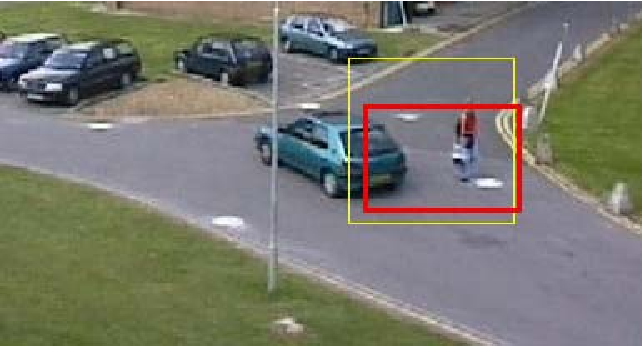
\includegraphics[width=.45\textwidth]{figs/TRK_IPCV2009_PETS2001_FN_00592_outputGroundTruth}
				\label{fig:PETS2001_Frame592_Ground}
			}
		\subfigure[Base]
			{
				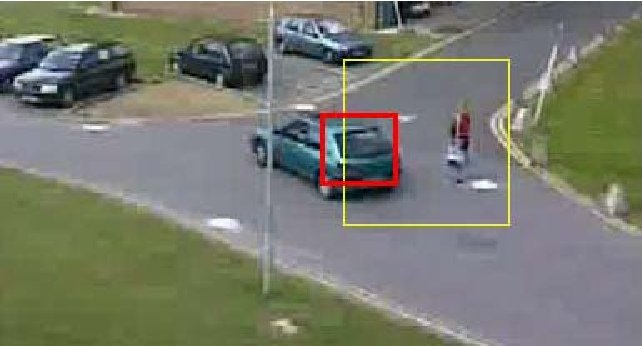
\includegraphics[width=.45\textwidth]{figs/TRK_IPCV2009_PETS2001_FN_00592_outputBaseline}
				\label{fig:PETS2001_Frame592_Base}
			}
		\subfigure[SigProc]
			{
				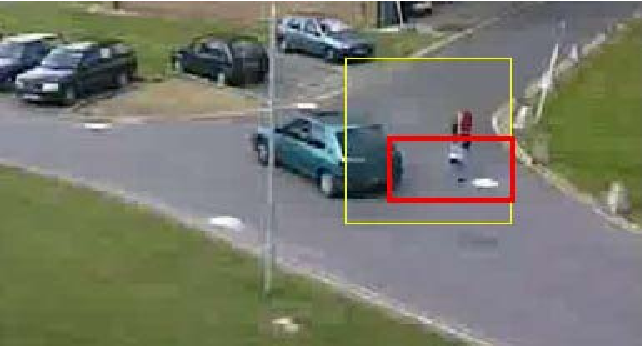
\includegraphics[width=.45\textwidth]{figs/TRK_IPCV2009_PETS2001_FN_00592_outputSigProc}
				\label{fig:PETS2001_Frame592_SigProc}
			}
		\subfigure[VarPar]
			{
				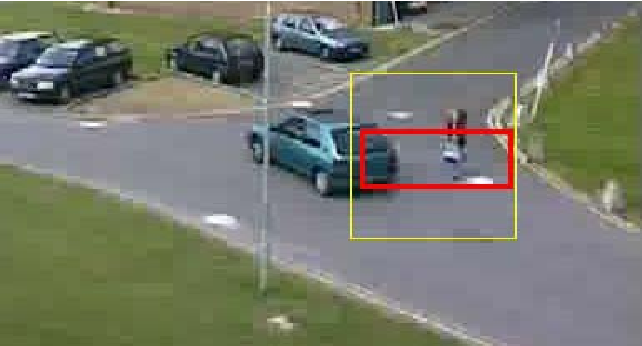
\includegraphics[width=.45\textwidth]{figs/TRK_IPCV2009_PETS2001_FN_00592_outputVarPar}
				\label{fig:PETS2001_Frame592_VarPar}
			}	
	\end{figure}
\end{frame}





\begin{frame}
\frametitle{Results}
\framesubtitle{PETS2007} 
\logoCSIPCPL\mypagenum
	\begin{itemize}
		\item object (bag) tracking
		\item dense background
		\item target occluded by object with similar color distribution
	\end{itemize}
	\begin{figure}
		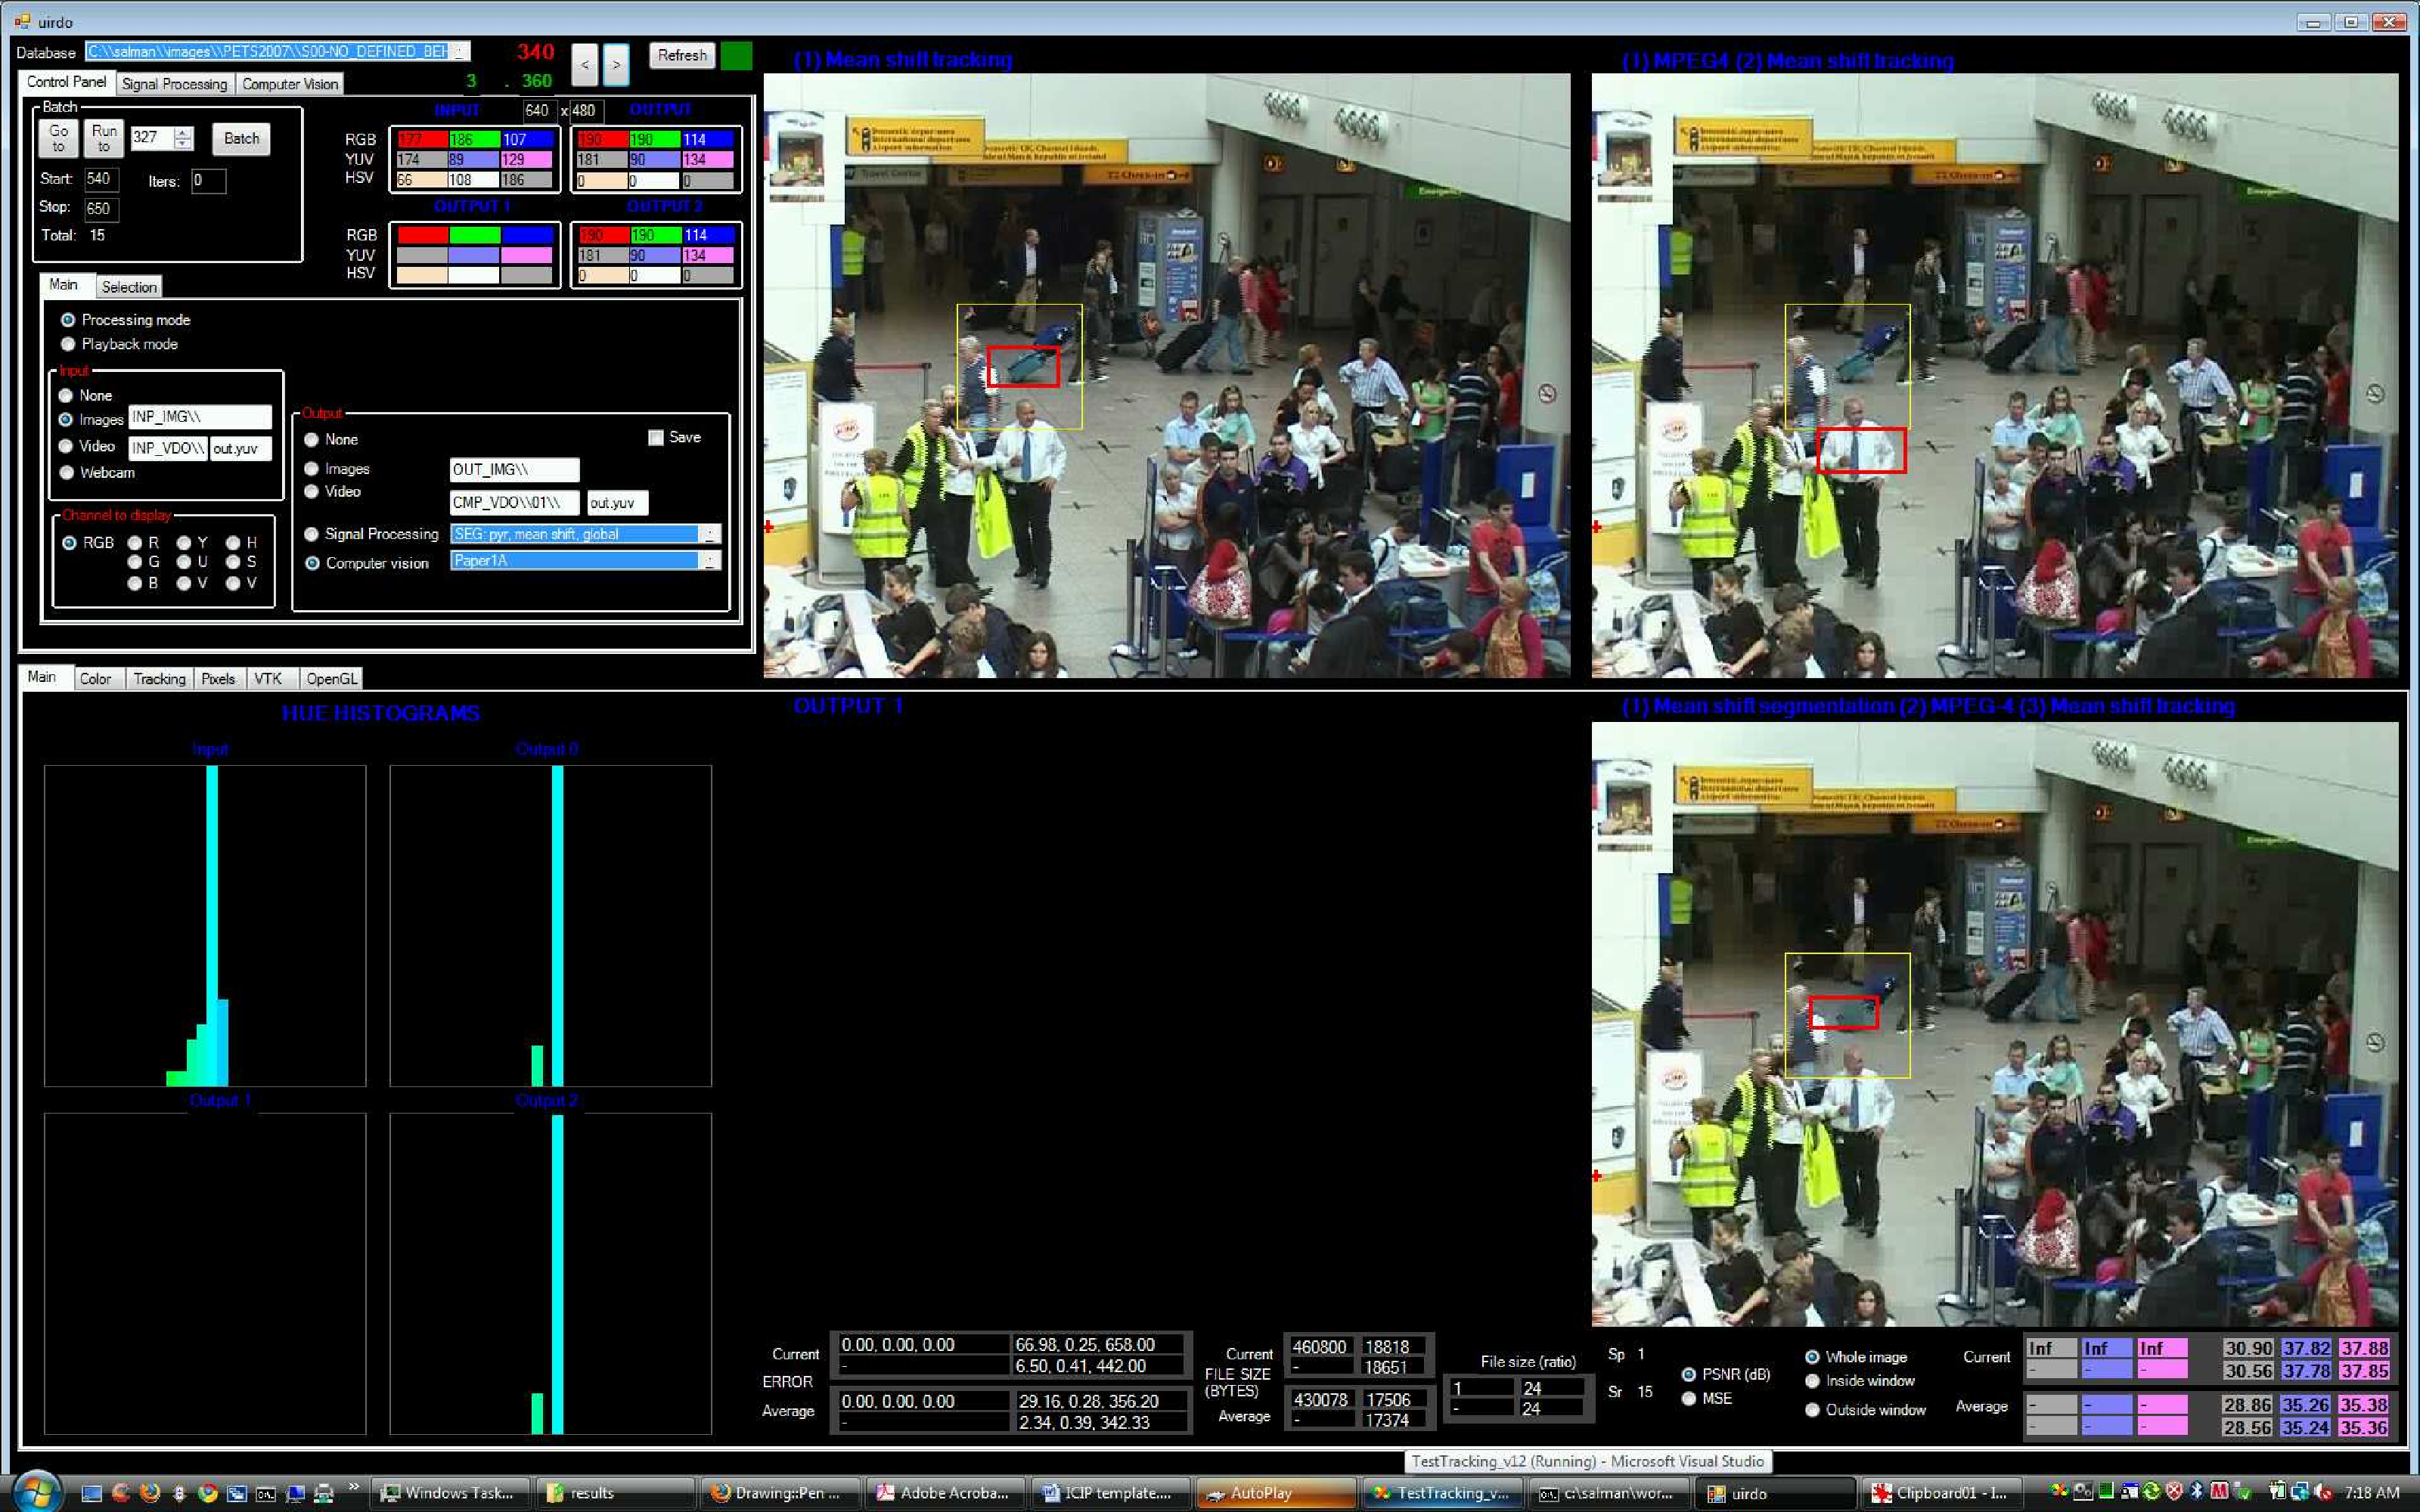
\includegraphics[width=1.0\textwidth]{figs/ICIP2009_PETS2007_FN_00340_snapshotVVG.pdf}
	\end{figure}
\end{frame}






\begin{frame}
\frametitle{Results}
\framesubtitle{PETS2007 (cont.)} 
\logoCSIPCPL\mypagenum
	\begin{figure}%[htp]
		\centering
		\subfigure[Ground truth]
			{
				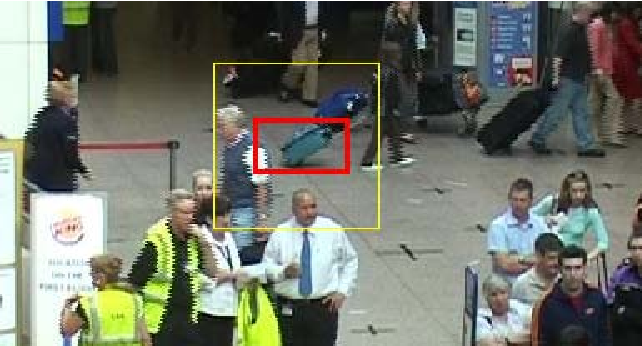
\includegraphics[width=.45\textwidth]{figs/TRK_IPCV2009_PETS2007_FN_00340_outputGroundTruth}
				\label{fig:PETS2007_Frame340_Ground}
			}
		\subfigure[Base]
			{
				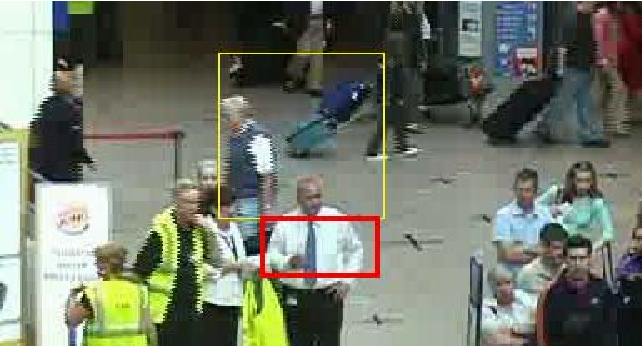
\includegraphics[width=.45\textwidth]{figs/TRK_IPCV2009_PETS2007_FN_00340_outputBaseline}
				\label{fig:PETS2007_Frame340_Base}
			}
		\subfigure[SigProc]
			{
				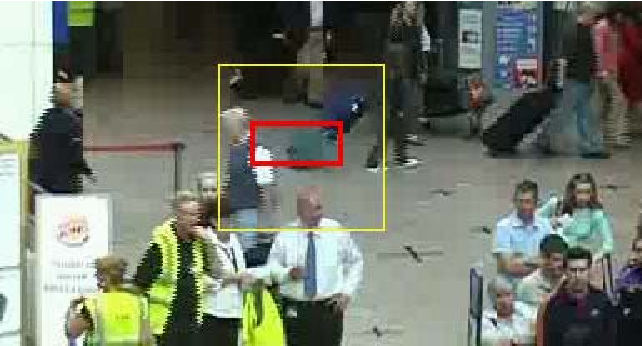
\includegraphics[width=.45\textwidth]{figs/TRK_IPCV2009_PETS2007_FN_00340_outputSigProc}
				\label{fig:PETS2007_Frame340_SigProc}
			}
		\subfigure[VarPar]
			{
				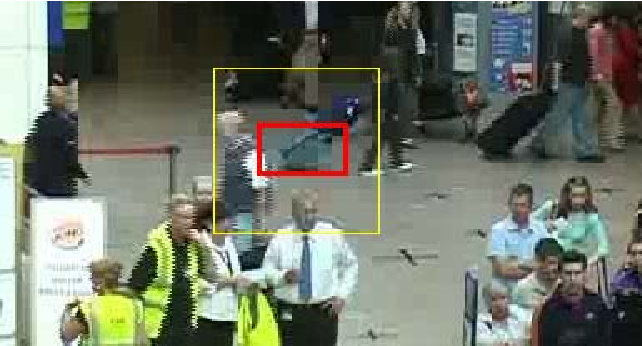
\includegraphics[width=.45\textwidth]{figs/TRK_IPCV2009_PETS2007_FN_00340_outputVarPar}
				\label{fig:PETS2007_Frame340_VarPar}
			}	
	\end{figure}
\end{frame}



\begin{frame}
\frametitle{Results}
\framesubtitle{tracking error: plotted against $Q_p$ and time, 3D}
\logoCSIPCPL\mypagenum
	\begin{figure}
		\centering
		\subfigure[PETS2001]
		{	
			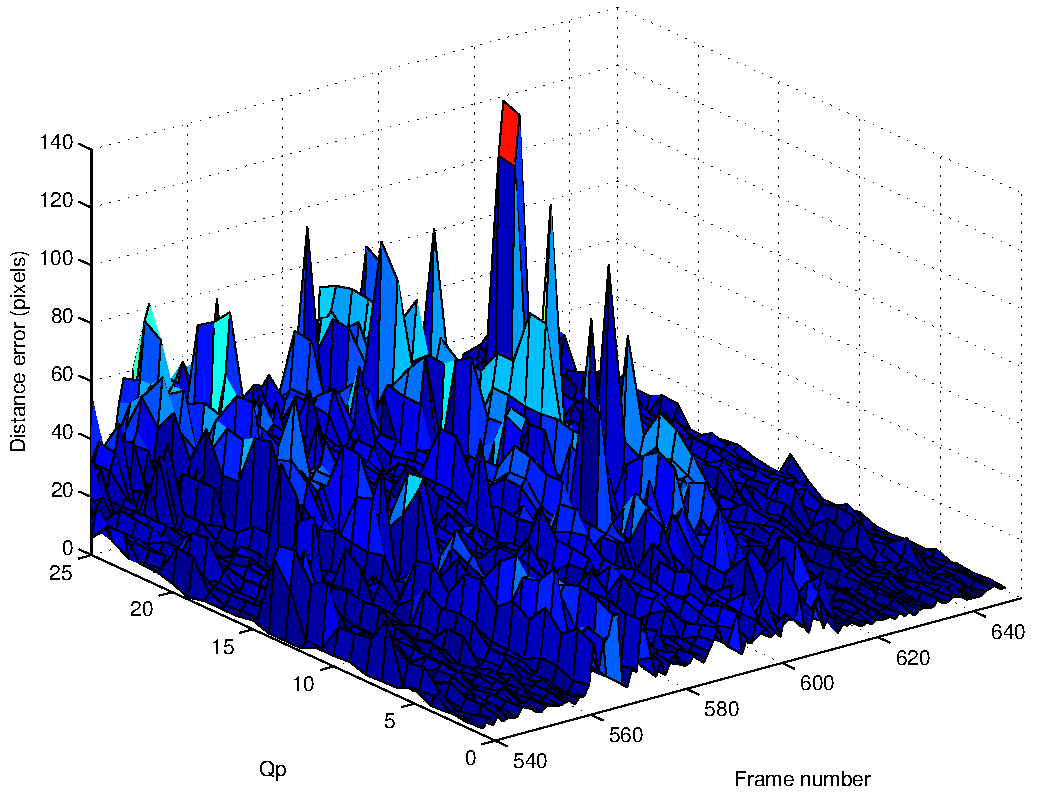
\includegraphics[width=.45\textwidth]{figs/TRK_IPCV2009_PETS2001_TrackingError3D}
		}
		\subfigure[PETS2007]
		{	
			\includegraphics[width=.45\textwidth]{figs/TRK_IPCV2009_PETS2007_TrackingError3D}
		}
		\caption{$VarPar$, tracking accuracy at different values of $Qp$.}
	\end{figure}
\end{frame}



\begin{frame}
\frametitle{Results}
\framesubtitle{tracking error: plotted against $Q_p$ and time, 2D}
\logoCSIPCPL\mypagenum
	\begin{figure}
		\centering
		\subfigure[PETS2001]
			{
				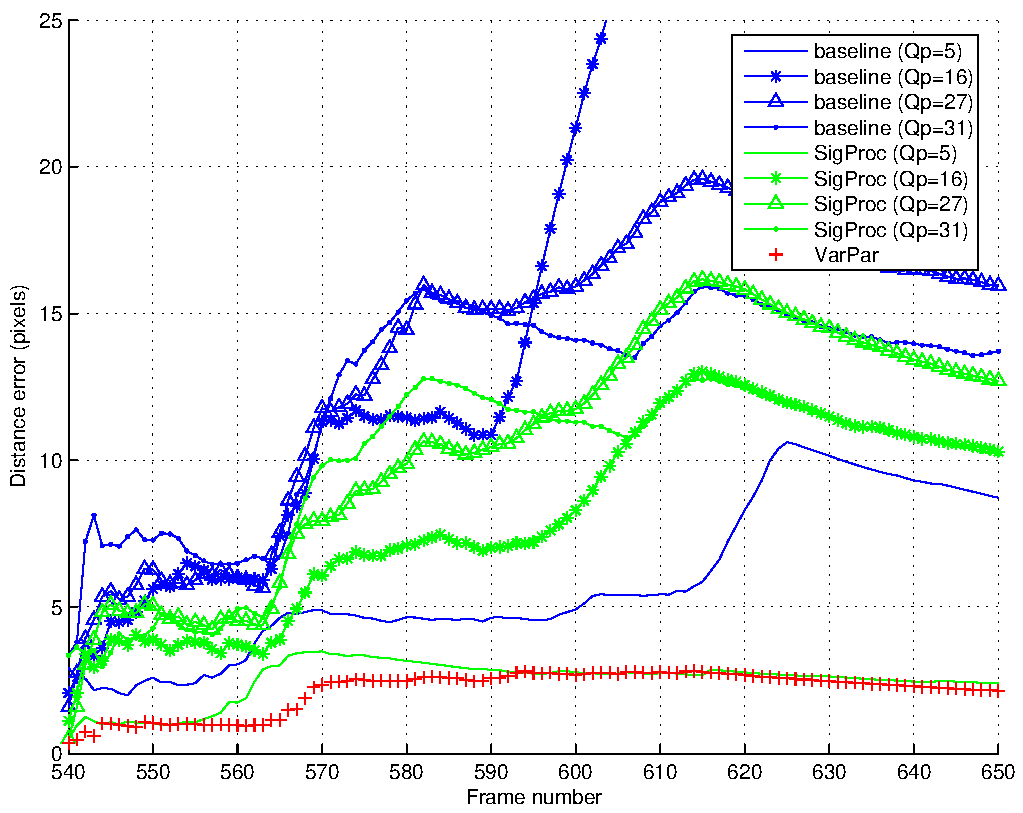
\includegraphics[width=.45\textwidth]{figs/TRK_IPCV2009_PETS2001_TrackingError}
			}
		\subfigure[PETS2007]
			{
				\includegraphics[width=.45\textwidth]{figs/TRK_IPCV2009_PETS2007_TrackingError}
			}
	\end{figure}
\end{frame}





\begin{frame}
\frametitle{Results}
\framesubtitle{tracking error: average over time and datasets}
\logoCSIPCPL\mypagenum
	\begin{figure}
		\includegraphics[width=1.0\textwidth]{figs/TRK_IPCV2009_TrackingErrorAllQp.pdf}
	\end{figure}
\end{frame}





\begin{frame}
\frametitle{Results}
\framesubtitle{tracking error: average over time}
\logoCSIPCPL\mypagenum
	\begin{table}
		\centering
		\begin{tabular}{|l|c|c|c|c|}
			\hline
			\multicolumn{5}{|c|}{Accuracy (distance from ground truth)} \\
			\hline
			Dataset & Qp & Baseline & $SigProc$  & $VarPar$\\ 
			\hline
			\multirow{4}{*}{PETS2001} 
				&5  & 8.7 	&   2.4 &   2.1 \\
				&16 & 75.4 &  10.3 &   2.1\\
				&27 &16.0 	&  12.7 &   2.1\\
				&31 &13.7 &  10.2 &   2.1\\
			\hline
			\multirow{3}{*}{PETS2007} 
				&5 &5.8 &   3.5 &   1.0\\
				&16 &85.1 &   4.2 &   1.0\\
				&27 &71.8 &   3.5 &   1.0\\
				&31 &15.2 &  35.8 &   1.0\\
			\hline
			\multirow{1}{*}{Average}
			& - & 36.5 & 10.3 & 1.6 \\  
			\hline
		\end{tabular}
	\end{table}
\end{frame}



%####################################################################################################
\section{Conclusions}
%####################################################################################################
\begin{frame}\frametitle{Conclusions} \logoCSIPCPL\mypagenum
	\begin{enumerate}
		\item It is possible to preserve information in a compressed video signal for a given application
			\begin{itemize}
				\item In this work, we focused on tracking at low bit-rates
				\item challenging scenes were used
				\item person or a bag was tracked after being occluded by another object with similar color distribution
			\end{itemize}
		\item Tracking accuracy was improved in 95 \% of the cases tested
			\begin{itemize}
				\item average PSNR drop of 5dB inside the segmentation window for a given bitrate
			\end{itemize}
	\end{enumerate}
\end{frame}


%####################################################################################################
%####################################################################################################
%\bibliographystyle{ieee}
%\bibliography{c:/salman/work/writing/MyCitations}
\end{document}
%####################################################################################################

%####################################################################################################

